\documentclass[letterpaper, 12pt]{math}

\usepackage{tikz}
\usetikzlibrary{arrows}

\title{University Physics 1A}
\author{Alvin Lin}
\date{September 6th, 2017}

\begin{document}

\maketitle

\section*{Kinematics}
Kinematics is the study of how things move. We study things by creating
mathematical models for the motions of objects. We model each of our objects
as a mass point.
\begin{center}
  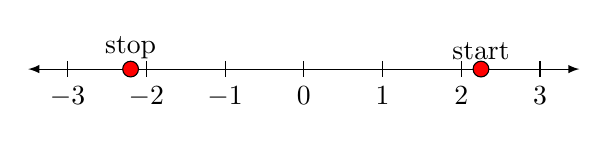
\begin{tikzpicture}
    \draw[latex-latex] (-3.5,0) -- (3.5,0) ; %edit here for the axis
    \foreach \x in  {-3,-2,-1,0,1,2,3} % edit here for the vertical lines
      \draw[shift={(\x,0)},color=black] (0pt,3pt) -- (0pt,-3pt);
    \foreach \x in {-3,-2,-1,0,1,2,3} % edit here for the numbers
      \draw[shift={(\x,0)},color=black] (0pt,0pt) -- (0pt,-3pt) node[below]
        {$\x$};
    \draw[fill=red] (-2.2,0) circle (0.1cm) node[above]{stop};
    \draw[fill=red] (2.25,0) circle (0.1cm) node[above]{start};
  \end{tikzpicture}
\end{center}
Displacement:
\begin{align*}
  \Delta x &= x_{final}-x_{initial} \\
  &= -2.2m-1.7m \\
  &= -3.9m
\end{align*}
The path length may be different from the displacement. The average speed is
how far it goes divided by how much time it takes. The average velocity is:
\[ \text{average velocity} = v_{avg} = \frac{\Delta x}{\Delta t} =
  \frac{x_{final}-x_{initial}}{t_{final}-t_{initial}} \]
\[ \text{instantaneous velocity} = v = \lim_{\Delta t\to0}\frac{\Delta x}
  {\Delta t} = \frac{\diff x}{\diff t} \]
Velocity measures how fast the position \( x \) is changing. It represents the
rate of change of position with respect to time.
\[ \text{average acceleration} = a_{avg} = \frac{\Delta v}{\Delta t} \]
\[ \text{instantaneous acceleration} = a = \lim_{\Delta t\to0}\frac{\Delta v}
  {\Delta t} = \frac{\diff v}{\diff t} = \frac{\diff^2 x}{\diff t^2} \]
Acceleration measures how fast the velocity \( v \) is changing.
\begin{align*}
  v &= \ddiff{x}{t} \\
  v\diff t &= \diff x \\
  \int_{t_0}^{t^1}v\diff t &= \int_{x_0}^{x^1}\diff x = x_1-x_0 \\ \\
  a &= \ddiff{v}{t} \\
  a\diff t &= \diff v \\
  \int_{t_0}^{t_1}a\diff t &= \int_{v_0}^{v_1}\diff v = v_1-v_0
\end{align*}
Complete the lab portion of the activities manual.

\section*{Reminders and Homework}
Complete the homework on TheExpertTA and WebAssign.

\begin{center}
  You can find all my notes at \url{http://omgimanerd.tech/notes}. If you have
  any questions, comments, or concerns, please contact me at
  alvin@omgimanerd.tech
\end{center}

\end{document}
